\section{Praxisteil}
% CRISP DM
% Hier noch mal beschreiben das lediglich der Effekt nachgewiesen werden soll, nicht belegt
% Im Zusammenhang mit Nutzung von Indizes erläutern (Grundlage rechtfertigen)

% Optimierung: Jeden Index in ein eigenes Cluster, dann Index weg

Im Praxisteil dieser Arbeit soll zuerst das Problem beschrieben und fachlich analysiert werden. Dazu gehört auch die Auswahl der Werkzeuge für die Umsetzung. Anschließend folgt die Strukturierung und Planung der Daten. Dies beinhaltet die Erstellung einer begründeten Datenstruktur. In dem Kapitel der \nameref{sec:datenvorbereitung} geht es dann um die Beschaffung, Aufbereitung und das Einlesen der Quelldaten in die Datenbank. Abschließend wird die Auswertung durchgeführt.

\subsection{Problemverständnis und Planung}
\label{sec:planung}
% Die konkreten Berechnungen hier einfügen
% Welche Daten werden benötigt?
% Welche Werkzeuge sollen genutzt werden (Wie sollen die Daten angezeigt werden um das Problem zu erläutern?)
% Mengen und Frequenzen von Daten

% anhand von großen Indizes um die Marktentwicklung insgesamt zu betrachten und nicht auf einzelne Aktien zu sehen
% In verschiedenen Ländern und Regionen (ob es Unterschiede gibt)
% Das soll über mehrere Zeiträume analysiert werden um wirklich eine Aussage treffen zu können
% Dazu werden die Daten historisch analysiert (soweit wie diese zurückgehen)
% Benötigt werden die täglichen Kursentwicklungen
% Berechnet wird die Kursentwicklung eines Tages mit der Formel (Schlusskurs Tag - Schlusskurs letzter Tag)
% Das ganze kann dann addiert werden nach Wochentagen um eine Gesamtstatistik zu erhalten

In dieser Auswertung soll untersucht werden ob der Weekend Effect in verschiedenen Regionen aufgetreten ist. Falls er existiert, ist ebenfalls interessant ob der Effekt je nach Zeitraum in der Vergangenheit unterschiedlich ausgeprägt war. Dafür werden historische Daten von yahoo Finance mit der Programmiersprache Python und der Datenbank OrientDB ausgewertet. Um bei der Auswertung möglichst die gesamte Entwicklung eines Marktes einzufangen und nicht Anomalien in den Kursverläufen einzelner Aktien zu untersuchen, werden dafür ausschließlich Daten von Aktienindizes verwendet. Benötigt werden dazu für jeden zu untersuchenden Index Daten in täglicher Frequenz. Diese sollten den Tagesschlusskurs, also den Kurs bei Schließung der Börse, und das Tagesdatum enthalten. Dann kann durch das Iterieren über alle Tage jeweils aus dem Schlusskurs des Vortages und dem Schlusskurs des aktuellen Tages die Differenz gebildet werden. Diese Differenzen nach Wochentagen summiert, ergeben dann die absoluten Kursveränderungen an den jeweiligen Tagen. Diese sollen anschließend mit der Python Bibliothek \enquote{matplotlib} visualisiert und verglichen werden.

% Bibliotheken
% Normalisierung der Ergebnisse?

\subsection{Datenverständnis}
% Datenstruktur und Format, Menge, Zeitauflösung etc.
% Was ist die ISIN?
% Wie und warum habe ich aufgebaut
% Adj_Close vs Close

% Daten kommen von yahoo Finance

Um die Daten für die Auswertung dauerhaft zur späteren Nachverfolgbarkeit zu behalten, wurde der Download als \gls{CSV} Datei statt der \gls{HTTP}-Schnittstelle gewählt. Es wurden Datensätze für die folgenden Aktienindizes gespeichert:

\begin{itemize}
    \item DAX (Deutscher Aktienindex) - Die größten 30 Unternehmen an deutschen Börsen. Daten seit 1987.
    \item Dow Jones Industrial Average - Die größten 30 Unternehmen an amerikanischen Börsen. Daten seit 1992.
    \item CAC40 - Die größten 40 Unternehmen an der Pariser Börse. Daten seit 1980.
    \item S\&P 500 - Die größten 500 Unternehmen an amerikanischen Börsen. Daten seit 1970.
    \item Euronext 100 - Die größten 100 börsennotierten Unternehmen aus den Ländern Frankreich, den Niederlanden, Belgien, Irland und Portugal. Daten seit 2000.
\end{itemize}

Für jeden Handelstag an der jeweils lokalen Börse existiert ein Datensatz. Neben den bereits genannten Daten wird ein bereinigter Tagesschlusskurs angegeben. Dieser rechnet Einflüsse wie Gewinnausschüttungen oder die Teilung von Aktien\footnote{Wenn ein Aktienpreis zu hoch steigt, kann das Unternehmen seine Aktien teilen. Bei einer 2:1 Teilung wird die Menge der Aktien verdoppelt und dafür der Preis halbiert. Aktien können auch andersherum zusammengeführt werden.} aus dem Schlusskurs heraus, um Kurssprünge zu vermeiden. Für die Datenanalyse werden lediglich das Datum, der Öffnungs- und bereinigte Schlusskurs benötigt.

% Wenn keine Ideen mehr Beispieldatensatz einfügen

\subsection{Datenbankvorbereitung}
% Einlesen der Daten und Aufbereitung
%   Behandeln von Ausreißern und fehlenden Daten zwischen den Datensätzen
%   Wie geht man mit unterschiedlicher Anzahl Wochentagen um? (Normalisierung)
% Format der Dokumente und Wahl der Tabellen
% ISIN
% CSV Format
% Schreiben der Daten in die Datenbank
% Erstellung des Datenbankindex
% Konfiguration

Um die Daten einlesen zu können, musste zuerst die Datenbank aufgesetzt werden. Diese wurde als Docker Container gehostet. Da es Inkompatibilitäten zwischen der Bibliothek PyOrient und der neusten Version von OrientDB gibt, wurde die Version 2.2.35 genutzt. Die Verbindungs- und Anmeldedaten werden zur Laufzeit des Python Skriptes aus einer Konfigurationsdatei geladen. Die Erstellung der Datenbank wird im Quellcode automatisiert. Dies ist im Listing \ref{list:create_db} zu sehen. In Zeile eins bis vier wird die Datenbank neu erstellt. Da hier unabhängige Datensätze ohne Verknüpfungen gespeichert werden sollen, wurde sich für das dokumentenbasierte Modell entschieden. Dies ist in Zeile vier bei der Erstellung der Datenbank zu sehen. Der Parameter \texttt{STORAGE\_TYPE\_PLOCAL} gibt an, dass der Inhalt auf der Festplatte gespeichert werden soll. Alternativ könnte OrientDB die Daten auch ausschließlich im Arbeitsspeicher halten. In Zeile sechs ist die Erstellung der neuen Klasse zu sehen. Die Variable \texttt{self.table\_index\_values\_name} ist ebenfalls in der Konfigurationsdatei definiert und gibt den Namen der Klasse an. Zusätzlich zur Klasse wird hier die Eigenschaft \texttt{Date} mit dem Datentyp \texttt{DATE} definiert. Dies gehört zum Schema der Klasse und wird benötigt, da OrientDB das Datumsfeld sonst als Zeichenkette interpretieren würde. Außerdem kann dann in Zeile acht ein Index auf das Datumsfeld gelegt werden, um Abfragen auf dieses zu optimieren. Mit der Angabe \texttt{NOTUNIQUE} wird ein SB-Tree Index erstellt, der doppelte Werte erlaubt. Dieser wurde gewählt, da bei mehreren Indizes Daten doppelt vorkommen können und auch Bereichsabfragen genutzt werden sollen.

\begin{figure}[!htb]
    \begin{lstlisting}[caption=Anlegen und initialiseren einer Datenbank in Python, label=list:create_db]
if self.client.db_exists(self.db_name):
    self.client.db_drop(self.db_name)

self.client.db_create(self.db_name, pyorient.DB_TYPE_DOCUMENT, pyorient.STORAGE_TYPE_PLOCAL)
self.database = self.client.db_open(self.db_name, self.username, self.password)
self.client.command("CREATE CLASS " + self.table_index_values_name + " IF NOT EXISTS")
self.client.command("CREATE PROPERTY " + self.table_index_values_name + ".Date DATE")
self.client.command("CREATE INDEX " + self.table_index_values_name + ".Date NOTUNIQUE")
    \end{lstlisting}
\end{figure}

\subsection{Datenvorbereitung}
\label{sec:datenvorbereitung}

Um die Einpflege der Daten zu automatisieren, wurde eine zweite Konfigurationsdatei mit einer Liste an Pfaden der einzelnen Dateien und eindeutigen Id's zu diesen angelegt. Beispielhaft ist der Eintrag des DAX in Listing \ref{list:config_dax} zu sehen. Als eindeutige Id, unter der später die Datensätze in der Datenbank getrennt gespeichert werden sollen, wurde die \gls{ISIN} gewählt. Diese stellt eine weltweit eindeutige Bezeichnung für Wertpapierprodukte dar.

\begin{figure}[!htb]
    \begin{lstlisting}[caption=Konfigeintrag des DAX, label=list:config_dax]
- file_name: "Index DAX Entwicklung.csv"
  isin: "DE0008469008"
    \end{lstlisting}
\end{figure}

Als nächstes wurde sich mit der Aufbereitung und dem Einpflegen in die Datenbank beschäftigt. Dies soll nach dem \gls{ETL} Prozess geschehen. Das bedeutet, zuerst werden die Daten aus der Ursprungsquelle extrahiert. Dann werden sie transformiert, also auf die spätere Nutzung angepasst. Als letztes werden die Daten in die Zieldatenbank geschrieben. Für das Auszulesen, wurde die Python Bibliothek \enquote{pandas} verwendet. Diese erlaubt das Lesen von tabellarischen Daten aus einer Vielzahl an Datenformaten und Quellen. Dafür wird durch die Liste der Datendateien in der Konfigurationsdatei iteriert. Jede Datei wird über den Befehl \texttt{pandas.read\_csv(path)} als DataFrame in den Arbeitsspeicher geladen. Die Daten können dann wie in Listing \ref{list:transformation} transformiert werden. Dazu gehört die Entfernung der Leerzeichen aus den Spaltennamen, wie in Zeile eins dargestellt. Diese sind in OrientDB nicht zulässig. Außerdem sollen, wenn verfügbar, immer die bereinigten Schlusskurse verwendet werden. Dafür werden die normalen Schlusskurse durch die Bereinigten, in Zeile drei und vier, überschrieben. Danach können dann alle nicht benötigten Spalten (Maximum, Minimum, doppelter bereinigter Schlusskurs und das Handelsvolumen) entfernt werden. Als letztes werden mit dem Befehl \texttt{dropna} alle Datensätze entfernt die einen oder mehrere fehlende Werte haben. Dies kommt bei den Daten von yahoo Finance gelegentlich vor. Mit diesen Datensätzen kann nicht gearbeitet werden.
% Tagesöffnungskurs bleibt drin

\begin{figure}[!htb]
    \begin{lstlisting}[caption=Transformation eines DataFrames, label=list:transformation]
df.columns = df.columns.str.replace(' ', '_')

if "Adj_Close" in df.columns:
    df["Close"] = df["Adj_Close"]

df.drop(['High', 'Low', 'Adj_Close', 'Volume'], axis=1, errors='ignore', inplace=True)
df.dropna(inplace=True)
    \end{lstlisting}
\end{figure}

Zum Schluss können die Daten in die Datenbank geschrieben werden. Um die Datensätze später wieder mit ihrer \gls{ISIN} zu verknüpfen, muss diese Information auch gespeichert werden. Üblicherweise würde eine neue Eigenschaft an jeden Datensatz angehängt, welche die \gls{ISIN} beinhaltet. Um die Suchperformance zu verbessern, könnte dann ein Datenbankindex auf dieses Feld erstellt werden. Durch die Nutzung von Clustern können Redundanzen der \gls{ISIN} und die Erstellung eines Index vermieden werden. Dazu wird bei der Speicherung der Datensätze der Befehl in Zeile zwei des Listings \ref{list:cluster_and_load} ausgeführt. Mit diesem wird je \gls{ISIN} ein neues Cluster erstellt. Die Suche nach Datensätzen kann dann sofort optimal auf ein Cluster eingegrenzt werden. Über den \texttt{INSERT} Befehl werden die Dokumente einzeln im \gls{JSON}-Format an die Datenbank übergeben und in das Cluster eingefügt.

\begin{figure}[!htb]
    \begin{lstlisting}[caption=Erstellung eines Clusters und Einfügen der Datensätze, label=list:cluster_and_load]
cluster_name = "index_" + isin
self.client.command("ALTER CLASS " + self.table_index_values_name + " ADDCLUSTER " + cluster_name)

for index, row in df.iterrows():
    insert_command = "INSERT INTO " + self.table_index_values_name + " CLUSTER " + cluster_name + " CONTENT " + row.to_json()
    self.client.command(insert_command)
    \end{lstlisting}
\end{figure}

% Eventuell noch Ausschnitt mit den Clustern aus Web-Interface

\subsection{Auswertung der Daten}
% Generierung der Auswertung mit Verweis auf das Problemverständnis
% Erstellung der Grafiken
% Zahlenoutput der Auswertung
% Problematisch wenn Daten fehlen? null, null, null etc.

Für die Auswertung der Daten soll die gesamte Entwicklung jedes Aktienindizes, nach Wochentagen aufgeteilt, visualisiert werden. Zusätzlich sollen auch 10-Jahres Zeiträume untersucht werden, um zu belegen das es sich nicht um eine zufällige Erscheinung handelt. Zehn Jahre wurden dabei gewählt um den Einfluss von kürzeren Börsenabstürzen minimal zu halten. In Listing \ref{list:manual_def} ist die Definition der Zeiträume im Python Code zu sehen. Beispielhaft werden hier einige Zeiträume des DAX und S\&P500 dargestellt. Da die Daten von yahoo Finance je nach Index unterschiedlich weit in die Vergangenheit reichen, wurden diese für jeden individuell angegeben.

\begin{figure}[!htb]
    \begin{lstlisting}[caption=Manuelle Definition der Untersuchungszeiträume, label=list:manual_def]
index_time_ranges = [
    IndexTimeRanges("DAX", "DE0008469008", [
        TimeRange("All time", "1970-01-01", "2022-12-31"), 
        TimeRange("1990 - 2000", "1990-01-01", "2000-12-31"), 
        ...
    ]),
    IndexTimeRanges("S&P500", "US78378X1072", [
        TimeRange("All time", "1970-01-01", "2022-12-31"), 
        TimeRange("1970 - 1980", "1970-01-01", "1980-12-31"), 
        ...
    \end{lstlisting}
\end{figure}

Die Auswertung wurde wie im \cref{sec:planung} berechnet. Dafür wurde die in Listing \ref{list:calc_auswertung} abgebildete Funktion geschrieben. Diese summiert unter Angabe eines Wochentages und ob die positive oder negative Entwicklung betrachtet werden soll alle Tageskursentwicklungen der übergebenen Daten. Dabei müssen die Tage wie in Zeile fünf angegeben, nach ihrem Datum sortiert, durchlaufen werden. Ansonsten könnte nicht die Differenz aus Schlusskurs und Schlusskurs des letzten Eintrags in der Schleife berechnet werden. Der letzte Schlusskurs wird dabei in der Variablen \texttt{last\_close} festgehalten. Für den ersten Eintrag wird die Differenz aus dem Schlusskurs und dem Öffnungskurs verwendet (siehe Zeile sieben).

\begin{figure}[!htb]
    \begin{lstlisting}[caption=Berechnung der Kursentwicklung nach Wochentag, label=list:calc_auswertung]
def __sum_value_changes(data, weekday, positive_change):
    last_close = 0
    value = 0

    for d in sorted(data, key=operator.attrgetter('date')):
        if d.date.weekday() == weekday:
            curr_value = d.close - last_close if last_close != 0 else d.close - d.open

            if positive_change and curr_value >= 0:
                value += curr_value
            elif not positive_change and curr_value < 0:
                value += curr_value

        last_close = d.close

    return value
    \end{lstlisting}
\end{figure}

In der Tabelle \ref{tab:ausw_sp500} ist eine beispielhafte Auswertung, die mit der Funktion aus Listing \ref{list:calc_auswertung} erstellt wurde. Diese wurde für den S\&P 500 und den Zeitraum vom 01.01.1970 bis zum 24.06.2021 erstellt. Die Eigenschaften \texttt{total\_pos} und \texttt{total\_neg} beschreiben die absolute positive bzw. negative Entwicklung an den Wochentagen. \texttt{total} ist die Summe der beiden und gibt damit die gesamte Kursveränderung an. Hier ist zu sehen das sich der Kurs des Index entsprechend des \enquote{Weekend Effect} tatsächlich montags mit 411,6461 Punkten am schlechtesten entwickelt hat. Allerdings liegt der Donnerstag mit 561,4188 Punkten sehr nah dran. Der beste Wert mit 1445,0413 Punkten tritt am Dienstag auf. Die Auswertung ist in grafischer Form im Anhang unter Abbildung \ref{fig:auswertung_sp500_graph} zu sehen.

\begin{table}[hbt]
    \centering
    \begin{minipage}[t]{1\textwidth} % Breite, z.B. 1\textwidth		
        \caption{Auswertung der Daten des S\&P500 im Zeitraum 01-01-1970 bis 24-06-2021} % Überschrift
        \begin{tabularx}{\columnwidth}{ |c|X|X|X|X| }
            \hline
            \textbf{weekday} & \textbf{total\_pos} & \textbf{total\_neg} & \textbf{total} \\ \hline
            Monday           & 8752,1193           & -8340,4732          & 411,6461       \\ \hline
            Tuesday          & 9697,5109           & -8252,4696          & 1445,0413      \\ \hline
            Wednesday        & 9207,6223           & -8129,4499          & 1078,1724      \\ \hline
            Thursday         & 9082,4919           & -8521,0731          & 561,4188       \\ \hline
            Friday           & 8901,1113           & -8131,5999          & 769,5114       \\ \hline
        \end{tabularx}
        \source{eigene Darstellung}
        \label{tab:ausw_sp500}
    \end{minipage}
\end{table}

Dieses Schema bestätigt sich auch wenn die beiden Zeiträume 1970 bis 1980 und 1980 bis 1990 betrachtet werden. Besonders deutlich wird dies in Abbildung \ref{fig:ausw_sp500_1970_1980}. Dort ist einzig Montags ein deutlich negativer Kursverlauf entstanden. Ein ähnliches Bild ist in Abbildung \ref{fig:ausw_sp500_1980_1990} im Anhang für den Zeitraum 1980-1990 zu sehen. Die etwas neuere Abbildung \ref{fig:ausw_sp500_1990_2000} zeigt allerdings das zwischen den Jahren 1990 und 2000 der Montag insgesamt der stärkste Tag war. Auch in dem Zeitraum 2000 bis 2010 lag der Montag, wie im Anhang in Abbildung \ref{fig:ausw_sp500_2000_2010} zu sehen, eher im Mittelfeld. Dies spricht gegen den Effekt.

\begin{figure}[!htb]
    \centering
    \begin{minipage}[t]{.48\textwidth}
        \caption{Auswertung S\&P500 - 70er}
        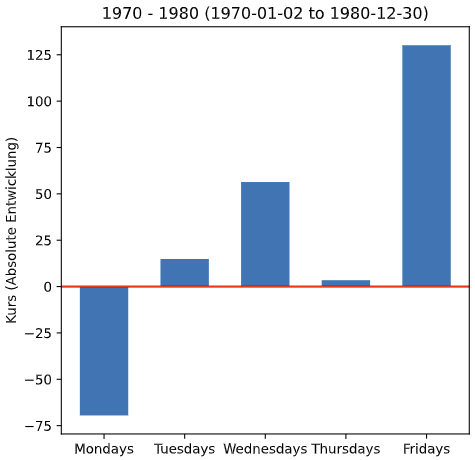
\includegraphics[width=1\textwidth]{img/Auswertung_SP500_1970-1980.PNG}\\
        \source{eigene Darstellung}
        \label{fig:ausw_sp500_1970_1980}
    \end{minipage}%
    \
    \begin{minipage}[t]{.48\textwidth}
        \caption{Auswertung S\&P500 - 90er}
        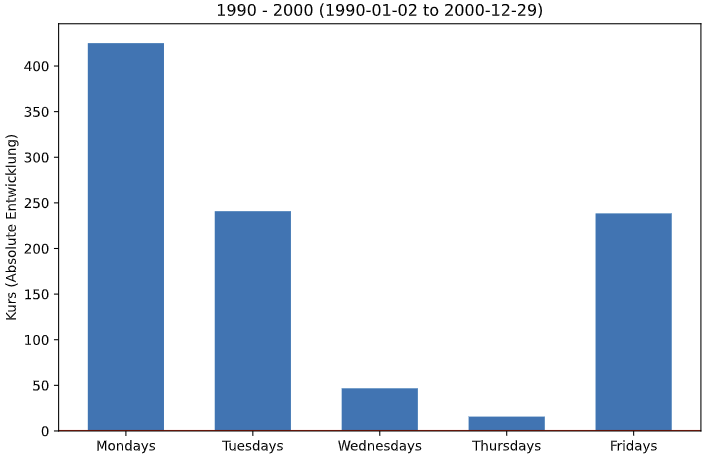
\includegraphics[width=1\textwidth]{img/Auswertung_SP500_1990-2000.PNG}\\
        \source{eigene Darstellung}
        \label{fig:ausw_sp500_1990_2000}
    \end{minipage}
\end{figure}

Bei den anderen Indizes ist zu beobachten, dass der Montag sowohl für den DAX als auch den Dow Jones Industrial in den untersuchten Zeiträumen nie der schlechteste Tag war. Für den CAC40 waren die Ergebnisse uneindeutig. Der Euronext 100 hingegen zeigt die Auffälligkeit, dass der Montag bei zwei von vier Ergebnissen am schlechtesten ausfiel, aber dafür in jedem Zeitraum negativ verlief.

\clearpage